% This is samplepaper.tex, a sample chapter demonstrating the
% LLNCS macro package for Springer Computer Science proceedings;
% Version 2.21 of 2022/01/12
%
\documentclass[runningheads]{llncs}
%
\usepackage[T1]{fontenc}
% T1 fonts will be used to generate the final print and online PDFs,
% so please use T1 fonts in your manuscript whenever possible.
% Other font encondings may result in incorrect characters.
%
\usepackage{graphicx}
\usepackage{amsmath}
\usepackage{booktabs}   % for nice tables
\usepackage{algorithm}
\usepackage{algpseudocode}
\usepackage{tabularx}
\usepackage{booktabs}
\usepackage{listings} % check to use recommended package
\usepackage[colorlinks=true, linkcolor=blue, urlcolor=cyan,
pdfpagemode=UseOutlines]{hyperref} % check if it is correct to use
% this
\hypersetup{bookmarksdepth=4}
% Manage acronyms
\usepackage[nolist]{acronym}
\usepackage{dirtytalk}
\usepackage{mismath}
\usepackage{amsmath}
\usepackage{amssymb}
% \usepackage{tikz}
% \usetikzlibrary{shapes.geometric, arrows.meta, positioning}
\usepackage{numprint}
\usepackage{multirow}
\usepackage{threeparttable}
\usepackage{subcaption}
\usepackage{adjustbox}
% -------------------- thesis transfer learning equation
% --------------------
\DeclareMathOperator{\ypred}{\phi}  %options \hslash
\DeclareMathOperator{\ypredtarget}{\phi^{T}}
\DeclareMathOperator{\ypredsource}{\phi^{S}}
\DeclareMathOperator{\ConvNetOut}{\mathcal{A}}
% --------------------++--------------------
% Used for displaying a sample figure. If possible, figure files should
% be included in EPS format.
%
% If you use the hyperref package, please uncomment the following two lines
% to display URLs in blue roman font according to Springer's eBook style:
%\usepackage{color}
%\renewcommand\UrlFont{\color{blue}\rmfamily}
%\urlstyle{rm}
%

% ==================== IMRAD ====================
% 1. **I**ntroduction  
% 2. **M**ethods  
% 3. **R**esults  
% 4. **A**nd  
% 5. **D**iscussion  

% ==================== General Writing Tips ====================

% - Keep sentences clear and direct.
% - Use past tense for methods/results, present tense for facts.
% - Avoid redundancy; be precise with terminology.
% - Quantify performance improvements clearly.

% ==================== Prompts ====================
% You are computer science PhD professional. Your task is to assist me
% to improve the writing of scientific articles using academic tone and
% solving questions I have. The article is written in Latex so mastery
% in the use of Latex is expected.

\begin{document}
% Setting acronyms in paper
\begin{acronym}
  \acro{BC}[BC]{Breast Cancer}
  \acro{MG}[MG]{Mammography}
  \acro{TG}[TG]{Thermography}
  \acro{CAD}[CAD]{computer-aided detection}
  \acro{CNNs}[CNNs]{convolutional neural networks}
  \acro{ViTs}[ViTs]{Vision Transformers}
  \acro{ViT}[ViT]{Vision Transformer}
  \acro{FDA}[FDA]{Food and Drug Administration}
  \acro{SIT}[SIT]{Static Infrared Thermography}
  \acro{DIT}[DIT]{Dynamic Infrared Thermography}
  \acro{SLR}[SLR]{Systematic Literature Review}
  \acro{PICOC}[PICOC]{Population, Intervention, Comparison, Outcome,
    Context}
  \acro{DL}[DL]{Deep Learning}
  \acro{AI}[AI]{Artificial Intelligence}
  \acro{NLP}[NLP]{Natural Language Processing}
  \acro{TCN}[TCN]{Temporal Convolutional Network}
  \acro{TDL}[TDL]{Time Distributed Layers}
  \acro{RNN}[RNN]{Recurrent Neural Networks}
  \acro{HAR}[HAR]{Human Activity Recognition}
  \acro{ViViTs}[ViViTs]{Video Vision Transformers}
  \acro{ViViT}[ViViT]{Video Vision Transformer}
  \acro{IR}[IR]{Infrared}
  \acro{TM}[TM]{Temperature Maps}
  \acro{LSTM}[LSTM]{Long Short Memory}
  \acro{UFF}[UFF]{Universidade Federal Fluminense}
  \acro{AUC}[AUC]{Area Under the Receiver Operating Characteristic
    Curve}
  \acro{lr}[lr]{learning rate}
  \acro{TL}[TL]{Transfer Learning}
  \acro{FT}[FT]{Fine-Tuning}
\end{acronym}

% 
% \title{Transformer-based Breast Cancer Thermography Detection} 
\title{Video Transformers for Dynamic Breast Infrared Imaging Classification}
%
%\titlerunning{Abbreviated paper title}
% If the paper title is too long for the running head, you can set
% an abbreviated paper title here

% 
\author{Lenin G. Falconi\inst{1}\orcidID{0000-0003-4402-6643} \and
  Maria Pérez\inst{1}\orcidID{0000-0003-0942-673X} \and
  Marco E. Benalcázar\inst{1}\orcidID{0000-0002-5275-7262} \and 
Aura Conci\inst{2}\orcidID{0000-0003-0782-2501}}
% a recomendation is to enter the hyperlinks to the orcid pages
% https://orcid.org/0000-0003-4402-6643 lenin falconi
% https://orcid.org/0000-0003-0782-2501 aura conci
% https://orcid.org/0000-0003-0942-673X maria pérez
% https://orcid.org/0000-0002-5275-7262 marco benalcazar
% 
\authorrunning{L. G. Falconi et al.}
% First names are abbreviated in the running head.
% If there are more than two authors, 'et al.' is used.
%
% \institute{Princeton University, Princeton NJ 08544, USA \and
% Springer Heidelberg, Tiergartenstr. 17, 69121 Heidelberg, Germany
% \email{lncs@springer.com}\\
% \url{http://www.springer.com/gp/computer-science/lncs} \and
% ABC Institute, Rupert-Karls-University Heidelberg, Heidelberg, Germany\\
% \email{\{abc,lncs\}@uni-heidelberg.de}}

\institute{Escuela Politécnica Nacional, Quito 170525, Ecuador\\
\url{https://www.epn.edu.ec} \\
\email{\{lenin.falconi,maria.perez, marco.benalcazar\}@epn.edu.ec} \and
Instituto de Computação, Universidade Federal Fluminense, Niterói – RJ
24210-346, Brazil\\
\url{https://www.ic.uff.br/}\\
\email{aconci@ic.uff.br}}
%
\maketitle              % typeset the header of the contribution
%
\begin{abstract}
% The abstract should briefly summarize the contents of the paper in
% 150--250 words.
  Breast Cancer is a leading cause of mortality among women
  worldwide and early detection remains crucial for improving patient
  survival rates. Thermography offers a non-invasive imaging
  technique for identifying abnormal temperature patterns associated
  with malignancies. In this work, we propose a video
  transformer-based model for automatic BC classification from
  thermographic images using Universidade Federal Fluminense
  dynamic acquisition protocol. Our model achieved an Area Under the
  Receiver Operating Characteristic Curve score of 0.94 on a
  test set of 15 patients outperforming the results of the
  state-of-the-art set by 3D Convolutional Neural Networks.
  % approach leverages transformers' capacity for modeling long-range
  % dependencies in image data, outperforming traditional \ac{CNNs}-based
  % methods on publicly available datasets. Experimental results
  % demonstrate superior accuracy, sensitivity, and specificity,
  % indicating the potential of attention mechanisms in medical image
  % analysis. These findings suggest that transformer-based models can
  % support clinicians in \ac{BC} screening workflows.

\keywords{Breast cancer detection \and Thermography \and Transformers \and Deep learning \and Medical image analysis.}
\end{abstract}

\section{Introduction}
\label{sec:introduction}
\ac{BC} remains one of the main health challenges affecting women
worldwide and it is the second most lethal form of cancer in
Ecuador~\cite{GLOBOCAN}. Since its introduction in 1960, \ac{MG} has
remained the gold standard for early detection
\cite{Kennedy2009,tsietso2022review}, with screening programs
demonstrating effectiveness in reducing mortality rates. However,
\ac{MG} faces limitations: reduced efficacy in younger women with
dense breast tissue, ionizing radiation risks, and reliance on manual
interpretation of low-contrast lesions with varied morphologies
\cite{Liu2023,Su2022}. In contrast, \ac{TG} offers a radiation-free,
non-invasive, and cost-effective alternative for \ac{BC} screening
that is applicable to all age groups without
contraindications. Moreover, when combined with machine learning
techniques, \ac{TG} demonstrates significant potential for early BC
detection~\cite{Rakhunde2022}.

Recent advances in \ac{AI}, particularly in \ac{DL}, have
significantly transformed \ac{CAD} systems for medical imaging
\cite{Litjens2017}. Although \ac{CNNs} currently dominate image
processing, emerging transformer-based models demonstrate superior
capabilities in global context modeling
\cite{dosovitskiy2020image}. This study investigates the application
of transformer architectures, specifically \ac{ViTs}, for automated
classification of \ac{BC} using the UFF's \ac{DIT} protocol, which
employs a sequence of temperature maps per patient
\cite{VisualLab2014}. This \ac{IR} image acquisition method
established the superiority of dynamic protocols for highlighting
vascular behavior~\cite{Silva2014}. In this work we hypothesize that
\ac{ViTs} can better model temporal dependencies in thermal sequences
compared to \ac{CNNs}. As a consequence, we examine both video and
image-based \ac{ViTs} implementations and compare their performance
with that of \ac{CNNs}-based architectures. Our primary objective is
to improve diagnostic accuracy in \ac{BC} classification through
\ac{TG} imaging. . The following are the proposed research questions
for this research:

\begin{enumerate}
\item \textbf{RQ1:} Do \ac{ViTs} outperform \ac{CNNs} in \ac{BC}
  classification from thermographic images due to their superior
  ability to model global contextual relationships?

\item \textbf{RQ2:} Does transfer learning with pre-trained \ac{ViTs}
  architectures improve classification accuracy compared to models
  trained from scratch for this medical imaging task?

\item \textbf{RQ3:} Does combining pre-trained \ac{ViTs} models with
  dynamic acquisition protocols enhance diagnostic classification
  performance for breast cancer detection in thermogram images
  compared to conventional approaches?
\end{enumerate}

% ==================== TO DO ====================
% This paragraph could be integrated to the previous 
In this work, we fine tune a \ac{ViViT} to classify thermal images
under the \ac{DIT} protocol. Our study makes the following key
contributions: (1) We extend \ac{ViT}-based approaches to \ac{DIT}
protocol, leveraging sequential image analysis to improve \ac{BC}
classification performance using a patient level dataset. (2) We
evaluate the impact of \ac{FT} using pre-trained \ac{ViTs}. (3) We
conduct experiments on two different versions of the DMR-IR dataset
(thermal map and thermal image) and compare performance to a simple
CNN architecture. (4) To the best of our knowledge, this is the first
study accounting the use of \ac{ViViTs} in \ac{DIT} protocol for
\ac{TG} in \ac{BC} classification. Our model achieved an
\ac{AUC}-score of $0.9350 \pm 0.0094$ in 10 fold cross validation
setup and 0.9444 on a separated test set of 15 patients with stratified
labels. This work advances the state-of-the-art set by
\cite{DeMatheus2023}, where 3D \ac{CNNs} achieved 93.51\% \ac{AUC} in
binary classification, and compliments the work by~\cite{Garia2023},
which achieved 95.7\% in \ac{SIT} protocol~\cite{Silva2014,VisualLab2014}.

The organization of this paper is presented as follows: In Section
\ref{sec:thermography}, a brief introduction to main characteristics
about the \ac{TG} protocols for screening BC is presented. Section
\ref{sec:literature-review} presents the related works to our research
questions. Our proposed methodology is presented in Section
\ref{sec:methodology}. Results are presented in Section
\ref{sec:results}. Finally, discussion over main findings is presented
in Section \ref{sec:discussion} and this work's conclusions in Section
\ref{sec:conclusions}.% and future works in \ref{sec:future-works}.

\section{Advantages of Dynamic Infrared Thermography in Breast Cancer}
\label{sec:thermography}
By acquiring the body's natural emissions of infrared radiation to map
the body's temperature distribution, \ac{TG} is a non-invasive imaging
modality that facilitates BC detection
\cite{Kennedy2009,Rakhunde2022,tsietso2022review}. Due to the
heightened metabolic activity of cancerous cells, there is an
increased blood flow to the tumor, which promotes the development of
new blood vessels presenting abnormal behavior under temperature
modifications. These anomalies typically appear as thermal
asymmetries between the contralateral sides in the breast region under
induced thermal stress. 

\begin{table}[!htbp]
\begin{threeparttable}
  \centering
  \caption{Comparison of \ac{MG} and \ac{TG}}
  \label{tab:mg-tg-compare}
  \scriptsize
  % \footnotesize
  \begin{tabularx}{.9\textwidth}{XXX}
    \hline
    \textbf{Parameter} & \textbf{Mammography} & \textbf{Thermography} \\
    \hline
    Basis & X-rays & Infrared radiation \\
    Device & X-ray machine\footnote{includes compression system} & Infrared camera \\
    Output & Anatomical image & Thermal map \\
    Abnormality Type & Anatomical & Physiological \\
    Equipment cost & $\approx$
                     \$80K\tnote{a} & $\approx$ \$0.4K\tnote{b} \\
    Age & over 40 years & No age barrier \\
    Women with implants & Not so effective & Effective \\
    Breast Density & False Positives & Not affected \\
    Further Investigation & Unnecessary biopsies & Fewer biopsies\\
    Pain and Fear & Breast Compression & No touch\\
    Radiation & Ionizing radiation & None\\
    \ac{FDA} approval & Cancer diagnosis & Adjunct to MG\\
    \hline

  \end{tabularx}
  \begin{tablenotes}
  \item[a] https://www.blockimaging.com/
  \item[b] https://www.flir.com.mx

  \end{tablenotes}
\end{threeparttable}
\end{table}

Moreover, unlike \ac{MG}, which is less effective in younger patients
due to the characteristics of denser breast tissue, \ac{TG} can be
safely applied across all age groups and is generally more
cost-effective than \ac{MG} and other imaging modalities. It can also
be applied to females with dense breast tissue, women who are pregnant
or breast feeding. Although the \ac{FDA} approved \ac{TG} as a cancer
risk assessment tool in 1982, it is typically used as an adjunct to
\ac{MG} rather than a standalone diagnostic
method~\cite{Kennedy2009,Ryan2025}. Advances in thermal sensing
equipment, image processing, machine learning and \ac{AI} pipelines
have contributed to more feasible and accurate \ac{CAD} systems for
infrared \ac{TG}.

\ac{TG} images can be obtained by using two different protocols:
\ac{SIT} and \ac{DIT}. The former consists in capturing the thermal
images under controlled conditions of frontal, oblique and lateral
breast views~\cite{Ryan2025}. The latter measures the thermal response
to a thermal stress applied to the
patient~\cite{Ryan2025,tsietso2022review}. The UFF's \ac{DIT} protocol
captures an image every 15 seconds over an interval of 5 minutes,
resulting in a sequence of 20 images per
patient~\cite{DeMatheus2023,VisualLab2014}. Despite its advantages, \ac{TG} is
susceptible to procedural inconsistencies and thermal noise
interference. A major challenge lies in the non-specificity of thermal
anomalies, which complicates accurate interpretation. For instance,
elevated temperatures may result from non-cancerous conditions such as
infections or inflammations. A comparative overview of \ac{TG} and
\ac{MG} is presented in Table \ref{tab:mg-tg-compare}.

\section{Approaches for Sequence Modeling}
\label{sec:appr-sequ-model}

\subsection{Image Vision Transformers}
\label{sec:vision-transformers}

In 2017, the Transformer architecture was introduced in the seminal
paper \say{Attention Is All You Need} as the first sequence
transduction model relying entirely on attention mechanisms
\cite{NIPS2017_3f5ee243}. This architecture replaced recurrent layers
with an encoder-decoder structure based on multi-head self-attention,
establishing itself as the state-of-the-art approach for \ac{NLP}
tasks.

Attention mechanisms had been previously explored in image processing
\cite{dosovitskiy2020image}. However, this work demonstrated that a
pure Transformer architecture could be directly applied to sequences
of image patches, treating them analogously to tokens in \ac{NLP}
tasks with minimal modifications to the original architecture. An
image patch, in a \ac{ViT} is a fundamental hyperparameter that
determines how an input image is divided into smaller segments
(patches) before being processed by the transformer architecture. The
patch size defines the dimensions of each non-overlapping block that
the image is split into. For an input image of size
\(H \times W \times C\) (Height × Width × Channels) and a patch size
of \(P \times P\), the number of patches is \(N = \frac{H}{P} \times
\frac{W}{P}\); where each patch becomes a token of dimension \(P
\times P \times C\). For instance, if the image is $(224 \times 224
\times 3)$, $N=\frac{224}{16}\times \frac{224}{16} = 14\times 14 =
196$ tokens.

Dosovitskiy et al. showed that \ac{ViTs} achieve
superior performance when pre-trained on large-scale datasets such as
ImageNet-21K and JFT-300M, followed by \ac{FT} for downstream
tasks, outperforming state-of-the-art \ac{CNNs}. Additionally, their
work provides key implementation insights: (1) \textbf{Positional
  embeddings} show no significant improvement when extended to 2D
representations; (2) \textbf{\ac{FT}} employs higher-resolution
images while maintaining original patch size~\cite{Kolesnikov2019};
(3) \textbf{\ac{TL}} replaces the classification head with a
zero-initialized linear layer matching the target output dimension;
(4) \textbf{Training} requires strong regularization for scratch
training on ImageNet with cosine learning rate decay; (5)
\textbf{Preprocessing} adheres to guidelines from
\cite{Kolesnikov2019}. 

\subsection{Video Transformers}
\label{sec:video-transformers}
Video can be understood as a sequence of images through a time
dimension that introduces motion and deformations on them
\cite{Selva_2023}. Because of this sequential nature present in video
information, it would be expected that \ac{ViTs} to be effective in
video modeling~\cite{Bertasius2021}. The \textit{TimeSformer} stands
as the first convolution-free architecture that adapts the \ac{ViT}
architecture proposed in~\cite{dosovitskiy2020image} to video by
extending the self-attention mechanism from the image space to the
space-time 3D volum~\cite{Bertasius2021}. Their main idea is to treat
video as a sequence of patches extracted from the individual frames,
where each patch is linearly mapped into an embedding space with
positional information~\cite{Bertasius2021}.

There is active research on \ac{ViViTs}, with several notable
models proposed in recent literature (e.g., ViViT~\cite{Arnab2021},
MViT~\cite{Fan2021}). Most improvements across different architectures
primarily address the computational complexity inherent in Transformer
models, which scales quadratically with respect to the sequence length
$T$ (i.e., $\mathcal{O}(T^2)$). Additionally, these approaches tackle
challenges related to spatial redundancy, temporal fidelity, and
inductive biases~\cite{Selva_2023}.

\subsection{CNN-based Sequence Modeling}
\label{sec:sequence-modeling}
While \ac{RNN} architectures (e.g., LSTM and GRU) have traditionally
been the default choice for sequence modeling, recent studies suggest
that \ac{CNNs} may outperform them in certain tasks
\cite{Bai2018}. The \ac{TCN} is a general-purpose convolutional
architecture for sequence prediction characterized with two key
properties: (1) \emph{causal convolutions}, which prevent information
leakage from future to past data, and (2) a \emph{fixed output
  length}, enabling the model to map variable-length inputs to outputs
of the same length~\cite{Bai2018}.

A significant advantage of \ac{TCN} is its inherent parallelism, where
predictions for later time steps do not depend sequentially on earlier
ones. This is achieved by processing the same filter across each
layer, allowing the model to handle long input sequences efficiently
during both training and evaluation.

In contrast, Keras~\cite{chollet2015keras}, a popular \ac{DL}
framework, provides a \ac{TDL} wrapper that applies a given layer to
every temporal slice of an input. By reusing the same weights across
all timestamps in the 3D input tensor, this approach ensures parameter
efficiency. Recent work by~\cite{Dhage2025} demonstrates that
combining \ac{TDL} with LSTM can simultaneously improve feature
extraction and temporal pattern recognition in sequential data,
leading to enhanced accuracy in \ac{HAR} tasks.

% write something about 3D-CNN approaches

\section{Literature Review}
\label{sec:literature-review}

This section provides a systematic literature review following the
methodology proposed in~\cite{kitchenham2009systematic} to find
relevant works in the area of this research goals and questions.
To ensure comprehensive coverage of \ac{ViTs} and \ac{TG} applications, we
employed the \ac{PICOC} framework to engineer the search string. We focused
specifically on studies that combined thermographic imaging with
advanced computer vision techniques, particularly \ac{ViTs}, in the context of \ac{BC} detection.

\subsection{Search Methodology}
\label{sec:search-methodology}

We conducted targeted searches across four major digital libraries,
such as: ACM Digital Library, IEEE Xplore, Scopus, and Springer
Link. Additional repositories were examined but yielded no relevant
results aligned with our research scope. We employed the following
Boolean search query:

\begin{quote}
  \scriptsize
\texttt{(thermogram OR thermography) AND} \\
\texttt{(vision transformer OR vit) AND} \\
\texttt{(cnn OR convolutional neural networks OR deep learning OR machine learning) AND} \\
\texttt{(improve OR enhance) AND} \\
\texttt{(classification OR detection OR diagnosis OR segmentation) AND} \\
\texttt{breast cancer}
\end{quote} 

The search query was designed to identify research papers comparing
\ac{ViTs} and \ac{CNNs} models. Given the scope of our study, we
adopted broad inclusion criteria for \ac{DL}-based computer vision
models applicable to \ac{TG} image classification. We systematically
excluded studies that did not primarily focus on \ac{TG} as the
screening modality, such as those employing ultrasound, magnetic
resonance imaging, or \ac{MG}. Furthermore, non-specific sources
(e.g., journals containing multiple unrelated articles) were
discarded. During the search for \ac{BC} research, we also encountered
numerous studies on histopathological and genetic analyses, which were
outside our scope and thus excluded.

The execution of the proposed search strategy yielded 24 primary
studies after removing duplicates. Subsequently, each study underwent
a screening process where titles, keywords, and abstracts were
evaluated against the predefined inclusion and exclusion
criteria. This selection process resulted in 4 relevant publications
for the literature review. The scarcity of publications investigating
\ac{ViT} and \ac{TG} suggests significant opportunities for novel
contributions, with only one study~\cite{Garia2023} addressing
research objectives comparable to ours.

\subsection{Deep Learning for Dynamic Breast Thermography}
\label{sec:related-works-1}

According to our proposed search strategy for literature review, the
first study employing \ac{ViTs} for \ac{BC} classification using
\ac{TG} images is reported in~\cite{Garia2023}. Their approach
utilizes the standard \ac{ViT}-Base architecture with 12 layers, 12
attention heads, and a 768-dimensional embedding
spac~\cite{dosovitskiy2020image}. Similar to our work, their
methodology leverages the transformer's self-attention mechanism for
\ac{TG} image classification into \textit{Cancerous} or
\textit{Healthy} categories. The authors investigate the impact of
patch size on classification accuracy, demonstrating that
$32 \times 32$ patches yield superior performance compared to the
standard $16 \times 16$ configuration. Also, it is worth to mention
that their implementation does not incorporate pre-trained weights on
natural images or data augmentation techniques. Their approach
achieved an \ac{AUC} of 95.7\% for binary classification on the DMR-IR
datase~\cite{Silva2014}, using a total of 950 samples with an analysis
unit per \ac{TG} image. However, the study was limited to \ac{SIT}
acquisition protocol.

To benchmark our methodology against \ac{CNNs}-based approaches for
\ac{DIT}, we compare with~\cite{DeMatheus2023}, which employs
3D-\ac{CNNs} to recognize patterns changes in a sequence of \ac{TG}
images. Cancer identification using a sequence of images is similar to
action recognition and depend on spatio-temporal models that extract
space-time feature information from data. While 2D \ac{CNNs} applied
to individual frames remain competitive for action recognition
\cite{Tran2017}, 3D convolutions inherently capture motion information
across adjacent frames~\cite{Ji2013,Qiming2023}. In
\cite{DeMatheus2023}, each patient's data is represented as a
hypercube constructed by stacking 20 preprocessed frames. The
preprocessing stage involved the segmentation of the region of interest
from the original \ac{TG} images and their resized to
$32 \times 32\times 3$. Baffa et al. enhanced the model generalization
through data augmentation with the following operations: rotations up
to $15^\circ$, horizontal flips, shearing transformations and adding
noise. According to them, 3D CNN is capable of considering the spatial
relationships in each image and their evolution over a temporal
dimension. Their experiments employed the DMR-IR dataset, comprising
\numprint{2980} images from 149 patients. Under a K-fold
cross-validation strategy, their model achieved an \ac{AUC} score of
\(93.51\% \pm 4.03\%\).

Despite the current trend of researching modern \ac{DL} architectures
for \ac{BC} classification in infrared \ac{TG}, it should be noted
that texture-based \ac{CAD} systems can accurately classify \ac{BC} in
\ac{TG}, achieving over 90\% accuracy, due to the rich texture content
present in the images~\cite{Ryan2025}. A significant advantage of
these texture-based methods is their computational efficiency,
particularly when dealing with limited datasets, as they require
substantially fewer resources than their \ac{DL} counterparts. This
efficiency, however, comes at the cost of requiring manual feature
engineering, whereas \ac{DL} approaches automate the feature learning
process.

\section{Methodology}
\label{sec:methodology}

This section outlines the methodological procedures employed to
develop and validate our set of models for \ac{BC} using the \ac{DIT}
protocol, specially the efficacy of \ac{ViTs} models. The most similar
work to our approach was proposed in~\cite{Garia2023}, where the
authors trained a \ac{ViT} model from scratch using the same dataset
but the \ac{SIT} protocol. Their study does not evaluate the
performance of pre-trained \ac{ViTs}, which is studied now here.

From our literature review there is no previous automated
classification of \ac{BC} by using \ac{DIT} protocol and \ac{ViViTs}. To
benchmark our results, we consider the work of Baffa et al~\cite{DeMatheus2023},
where 3D \ac{CNNs} are employed to study the evolution of the sequence
of \ac{TG} images.

The methodology consists of seven main stages (Figure
\ref{fig:methodoly-overview}), where some steps vary depending on the
specific experiment. First, we formulated the machine learning
problem. Thereafter, we retrieved the sequences of \ac{TM}
($\mathbb{D}_{\mathrm{TM}} \in \mathbb{R}^{640 \times 480 \times 1}$) and
\ac{IR} images
($\mathbb{D}_{\mathrm{IR}} \in \mathbb{Z}^{640 \times 480 \times 3}$) for each
subject from the DMR-IR dataset, creating two distinct data
subsets. The \ac{TM} dataset comprises temperature matrices with a
precision of up to two decimal places and an accuracy of
\(0.02^\circ \text{C}\), whereas the \ac{IR} dataset consists of
three-channel RGB infrared images with pixel values ranging from 0 to
255.

Next, we set the preprocessing pipelines for each dataset
according to its specific characteristics, including data augmentation
during training. Afterward, for $\mathbb{D}_{\mathrm{IR}}$, we applied a
stratified holdout sampling technique, reserving 10\% of the cases as
a test set.  We then designed the models using a 5-dimensional input
tensor
$\mathcal{X} \in \mathbb{R}^{B \times F \times C \times H \times W}$,
where: $B$ denotes the batch size, $F$ represents the number of
frames, $C$ corresponds to the number of channels, and $H$ and $W$
indicate the height and width of the \ac{TM} or \ac{IR} images,
respectively. Due to the small dataset size, we evaluated the models
using \textit{K}-fold cross-validation. Finally, we selected the
best-performing model and evaluated it on the test set. We employed
AdamW as the optimizer together with checkpoint and early stopping
callbacks. All experiments were performed using Kaggle's GPU 1 x Tesla
P100 of 3584 CUDA cores, 16 GB GDDR6 and up to 30 GB of RAM.

% ==================== old flow chart methodology ====================
% \begin{figure}[ht]
%   \centering
%   \includegraphics[height=.6\textheight, width=\textwidth]{figures/methodology3.pdf}
%   \caption{Overview of the methodology used in this research. It
%     comprises seven stages: (1) Problem Formulation, (2) Data
%     Organization, (3) Preprocessing, (4) Data Patitioning, (5) Model
%     Design, (6) Model Training, and (7) Model Evaluation. \label{fig:methodoly-overview} }
%   \end{figure}

% ====================   new methodolgy figure but exceeds left margin ====================
% \begin{figure}[p]
% \centering
%   % Left column, top row
%   \begin{subfigure}[t]{\textwidth}
%     \centering
%     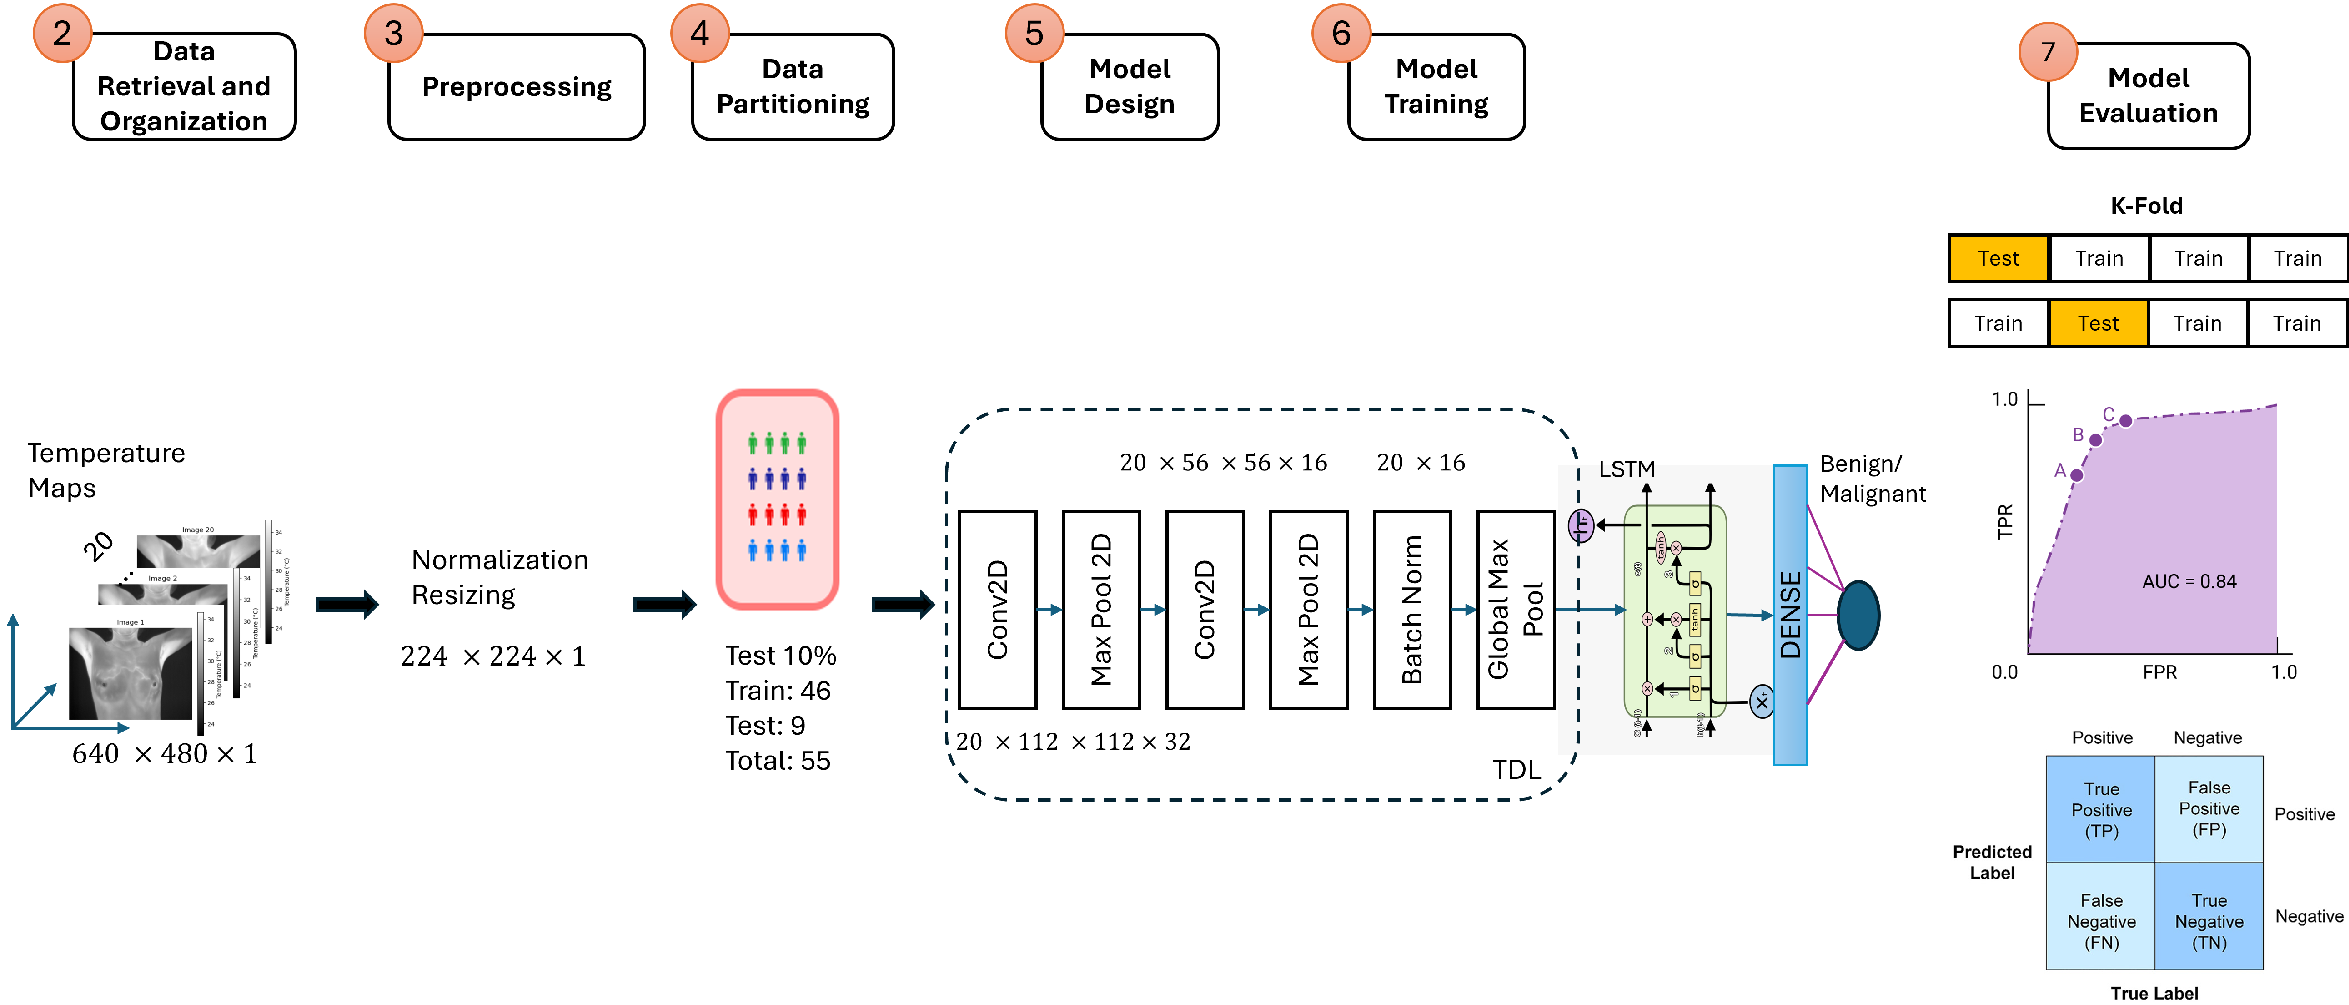
\includegraphics[width=1.3\linewidth, height=.48\textheight, keepaspectratio]{figures/methodology_TM.pdf}
%     \subcaption{Methodology for Temperature Maps: depicts the CNN
%       network with \ac{TDL}}
%     \label{fig:part1}
%   \end{subfigure}

%   % Left column, bottom row
%   \begin{subfigure}[t]{\textwidth}
%     \centering
%     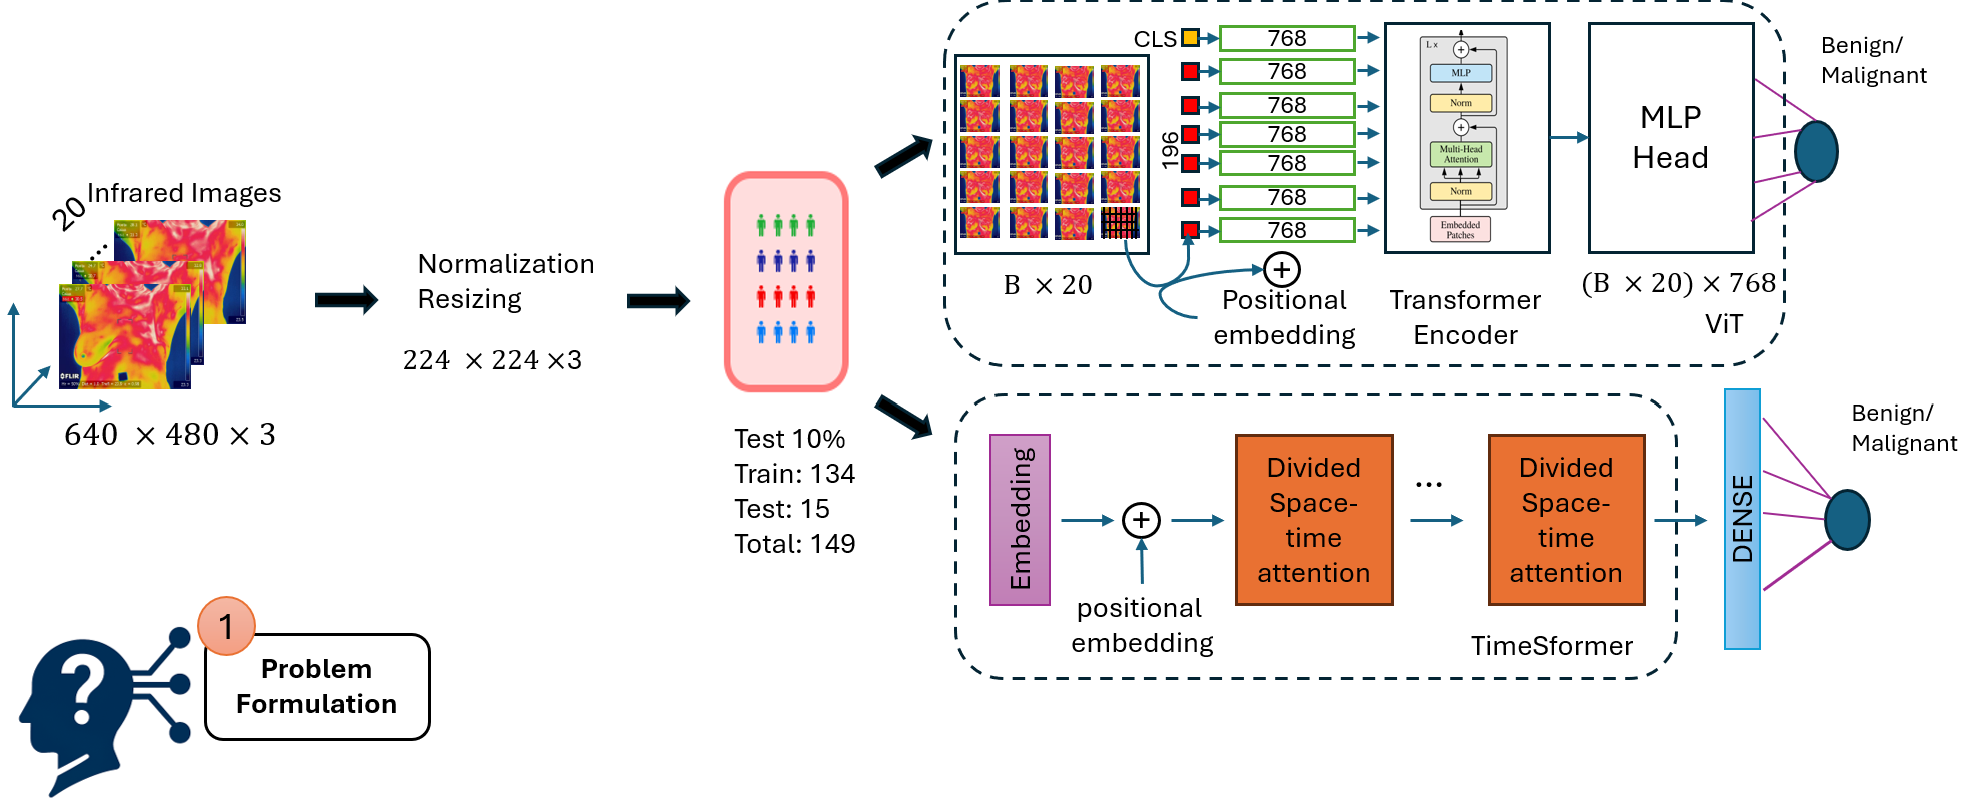
\includegraphics[width=1.3\linewidth, height=.48\textheight,keepaspectratio]{figures/Methodology_IR.pdf}
%     \subcaption{Methodology for Infrared Thermography Images: depicts
%       the \ac{ViT} and \ac{ViViT} models}
%     \label{fig:part2}
%   \end{subfigure}

% \caption{Overview of the methodology used in this research. It
%      comprises seven stages: (1) Problem Formulation, (2) Data
%      Organization, (3) Preprocessing, (4) Data Patitioning, (5) Model
%      Design, (6) Model Training, and (7) Model Evaluation for (a)
%      Temperature Maps and (b) Infrared Thermography Images }
% \label{fig:methodoly-overview}
% \end{figure}


\begin{figure}[p]
  \centering
  \begin{subfigure}[t]{\textwidth}
    \centering
    \makebox[\textwidth][c]{%
      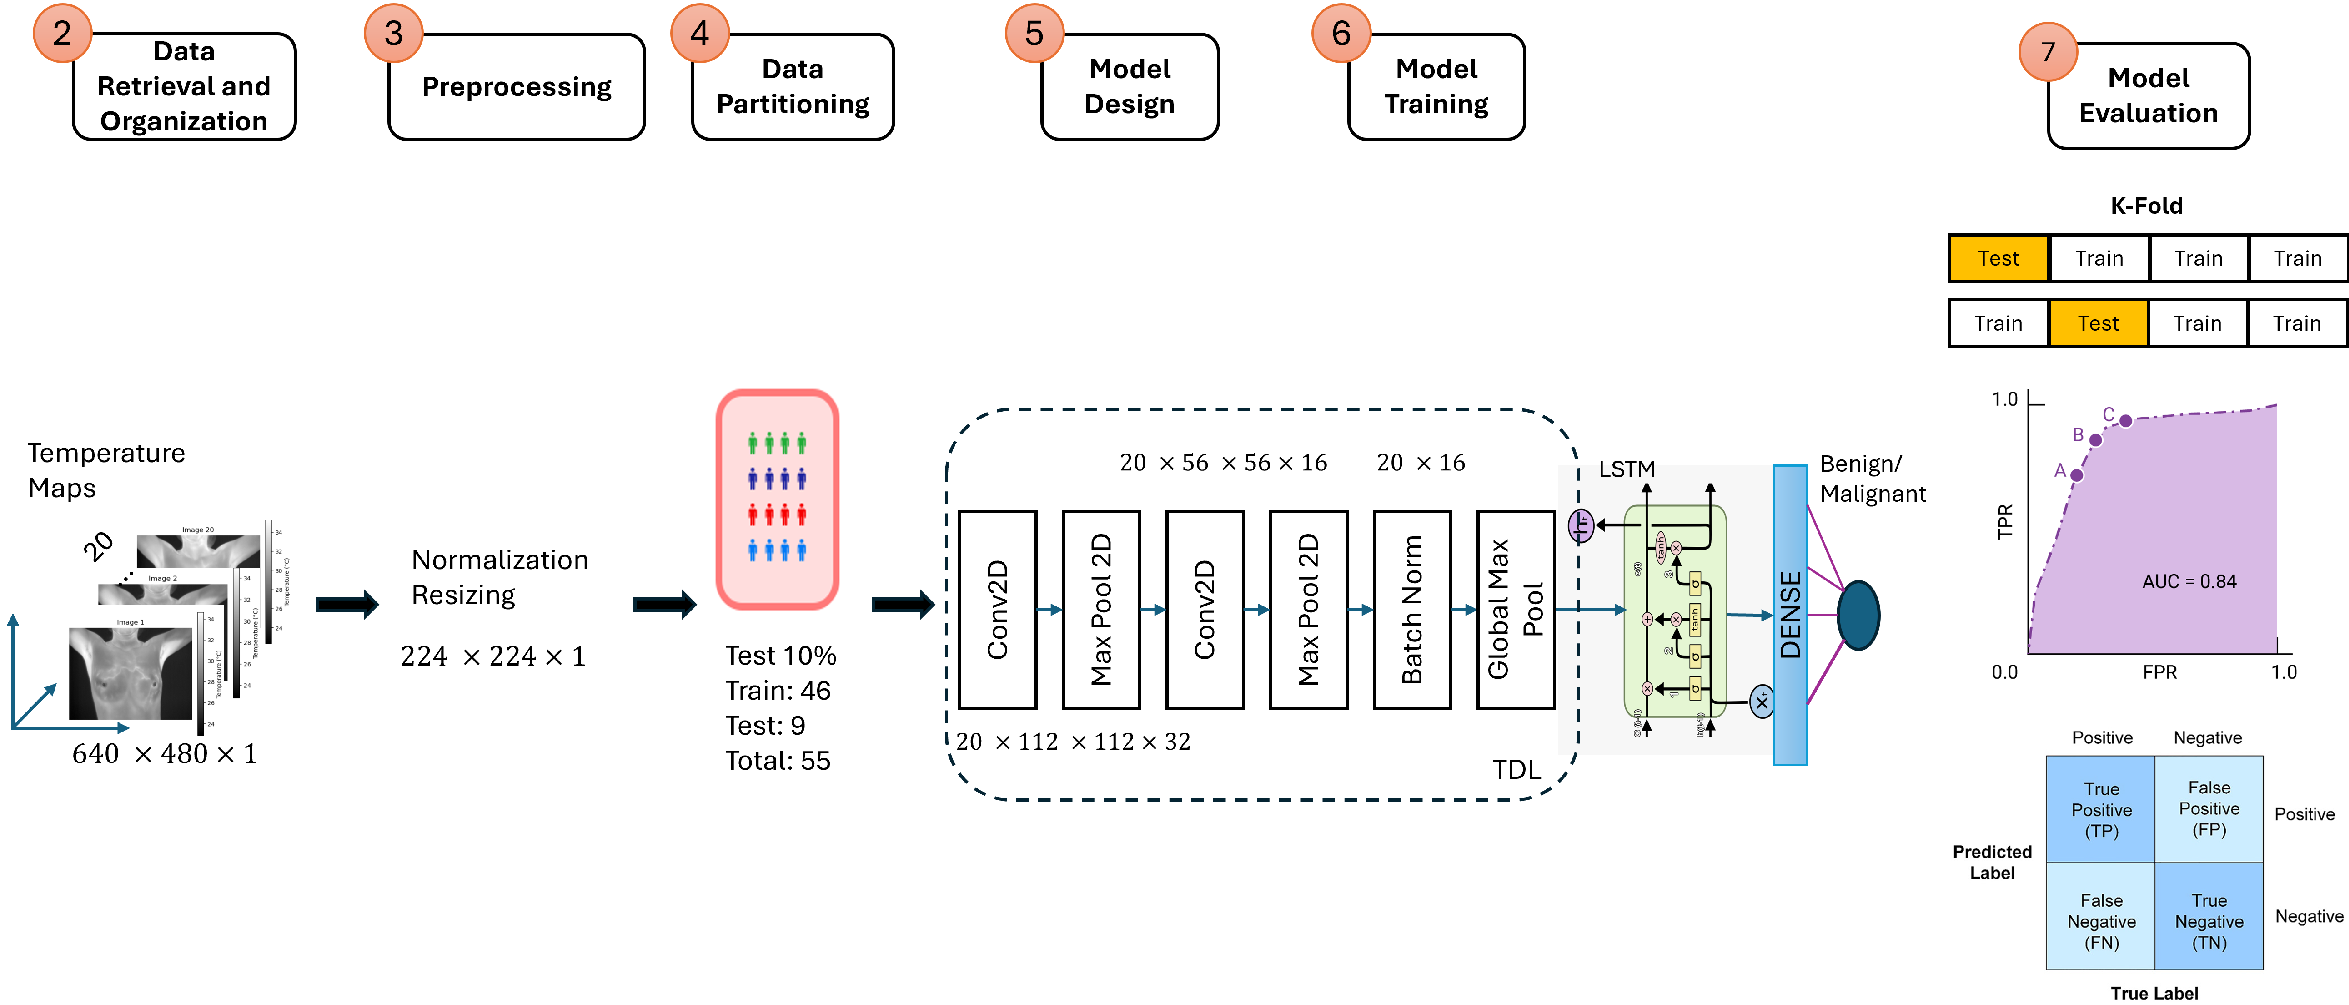
\includegraphics[width=1.2\textwidth, height=0.48\textheight]{figures/methodology_TM.pdf}%
    }
    \subcaption{Methodology for Temperature Maps: depicts the CNN
      network with \ac{TDL}}
    \label{fig:part1}
  \end{subfigure}

  \vspace{0.8em}

  \begin{subfigure}[t]{\textwidth}
    \centering
    \makebox[\textwidth][c]{%
      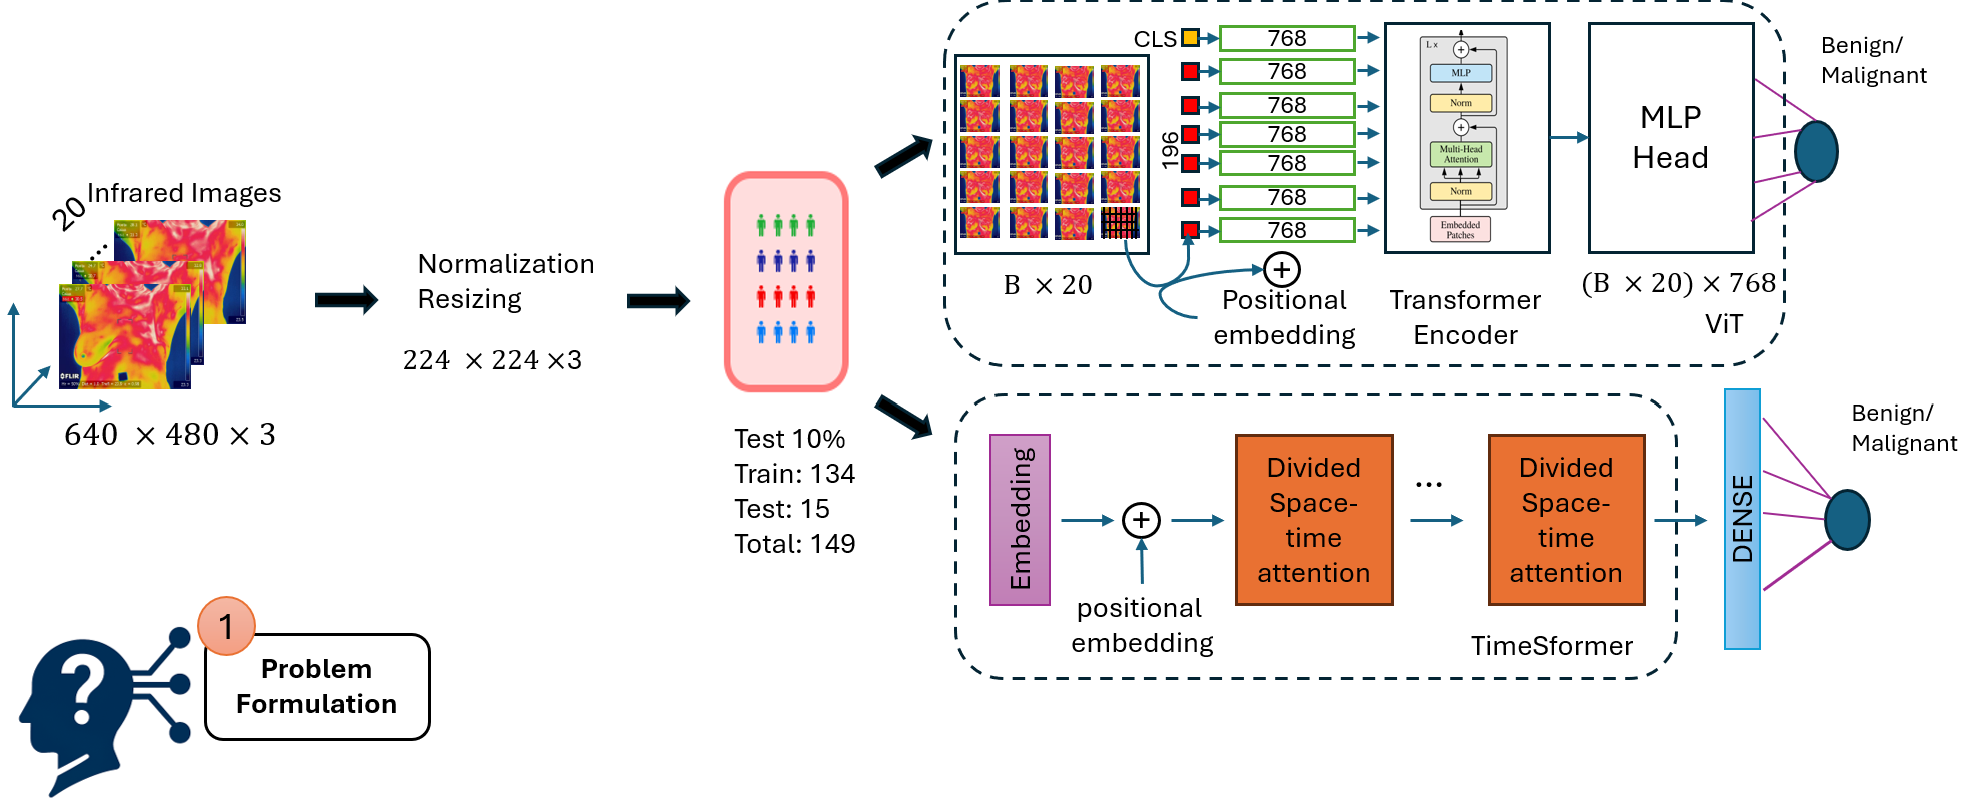
\includegraphics[ width=1.2\textwidth, height=0.48\textheight]{figures/Methodology_IR.pdf}%
    }
    \subcaption{Methodology for Infrared Thermography Images: depicts
      the \ac{ViT} and \ac{ViViT} models}
    \label{fig:part2}
  \end{subfigure}

  \caption{Overview of the methodology used in this research. It
     comprises seven stages: (1) Problem Formulation, (2) Data
     Organization, (3) Preprocessing, (4) Data Patitioning, (5) Model
     Design, (6) Model Training, and (7) Model Evaluation for (a)
     Temperature Maps and (b) Infrared Thermography Images.}
  \label{fig:methodoly-overview}
\end{figure}

\subsection{Problem Formulation}
\label{sec:problem-formulation}

Our objective is to train a model to classify a sequence of \ac{TG}
data into either \textit{Benign} or \textit{Cancer}. Consequently, we
want to find a mapping function
$f_{\theta}: \mathbb{R}^{F \times C \times H \times W} \to [0,1]$
with parameters $\theta$, where the predicted class probabilities for
an input sequence
$\mathbf{x} \in \mathcal{X} \subset \mathbb{R}^{F \times C \times H
  \times W}$:

\begin{equation}
    P(y = 1 \mid \mathbf{x}) = f_\theta(\mathbf{x}) \quad \text{(for $\mathbf{x} \in \mathcal{X}$)}
\end{equation}

Considering that a video classification aims to predict the class of a
given input sequence of frames~\cite{Selva_2023}, the final prediction
$\hat{y} \in \{0,1\}$ is:

\begin{equation}
    \hat{y} = \mathbb{I}\left( P(y = 1 \mid \mathbf{x}) \geq 0.5 \right)
\end{equation}
The optimization  minimizes the binary cross-entropy loss:
\begin{equation}
    \mathcal{L}(\theta) = -\frac{1}{N}\sum_{i=1}^N \left[y_i\log(\hat{y}_i) + (1-y_i)\log(1-\hat{y}_i)\right]
\end{equation}
where $y \in \{0,1\}$ are the ground truth labels.

In this context, we hypothesize that  \ac{ViViTs} can outperform
3D \ac{CNNs} in \ac{BC} classification for \ac{TG}.


\subsection{Model Fine-Tuning}\label{sec:transfer-learnin}
\ac{FT} is a \ac{TL} technique where the weights of a pre-trained model are further trained on a smaller, task-specific dataset. Typically, the classification head is replaced to adapt the model to the nuances of the new task. This process can update all layers of the pre-trained model or gradually unfreeze some of them (layer-wise fine-tuning). We adopt the formal definitions for \ac{TL} and \ac{FT} given in~\cite{falconi2020transfer}:

\begin{definition}[Transfer Learning]
  Given an original domain $\mathcal{D}^{S}$ with an original learning task $\mathcal{T}^{S}$, a target domain $\mathcal{D}^{T}$ with a target task $\mathcal{T}^{T}$, the transfer learning operation seeks to improve the learning of a prediction function $\ypredtarget(\cdot)$ in $\mathcal{D}^{T}$ using the knowledge acquired in $\ypredsource(\cdot)$ in $\mathcal{T}^{S}$, through $\phi^S$; where $\mathcal{D}^{S} \neq \mathcal{D}^{T}$ or $\mathcal{T}^{S} \neq \mathcal{T}^{T}$.
\end{definition}

Equations \eqref{eq:Transfer2} and \eqref{eq:Transfer3} represent the transfer learning operation and model prediction, respectively. Here, $L$ denotes the number of layers in the pre-trained model, and $\ConvNetOut$ refers to a set of operations that replace the original classification head.

\begin{equation}
  \mathbb{T}_{L} \left\langle \ypredsource(\mathcal{D}^{S}), \mathcal{D}^{T} \right\rangle = \ConvNetOut \left( \ypredsource(\mathcal{D}^{T}) \Bigr\rvert_{0}^{L} \right)
  \label{eq:Transfer2}
\end{equation}

\begin{equation}
  \mathcal{Y}^{T} = \mathbb{T}_{L} \left\langle \ypredsource(\mathcal{D}^{S}), \mathcal{D}^{T} \right\rangle = \ypredtarget(\mathcal{D}^{T})
  \label{eq:Transfer3}
\end{equation}

\begin{definition}[Fine-Tuning]
  Given an original domain $\mathcal{D}^{S}$ with an original learning task $\mathcal{T}^{S}$, a target domain $\mathcal{D}^{T}$ with a target task $\mathcal{T}^{T}$, the fine-tuning procedure enhances the learning of a target function $\mathcal{Y}^T = \ypredtarget(\mathcal{I}^T)$ by retraining $r$ layers of the original model $\mathcal{Y}^S = \ypredsource(\mathcal{I}^S)$ with $L$ layers, where $\gamma = L - r$.
\end{definition}

Equations \eqref{eq:finetuningLenin} and \eqref{eq:finetuningTunstall} represent the fine-tuning operation and the fine-tuned model prediction, respectively. Full model update occurs when $r = L$. The operation $\ConvNetOut$ involves replacing the original classification head of the pre-trained model. For instance, in the case of TimeSformer, it would replace the original 400-class output for Kinetics-400 with a new head appropriate for the target task.

\begin{equation}
  \mathbb{F}_{T} \left\langle \ypredsource(\mathcal{D}^{S}), \mathcal{D}^{T} \right\rangle = \ConvNetOut \left( \ypredsource \left( \ypredsource(\mathcal{D}^{T}) \Bigr\rvert_{0}^{\gamma - 1} \right) \Bigr\rvert_{\gamma}^{L} \right)
  \label{eq:finetuningLenin}
\end{equation}

\begin{equation}
  \mathbb{F}_{T} \left\langle \ypredsource(\mathcal{D}^{S}), \mathcal{D}^{T} \right\rangle = \ConvNetOut \left( \ypredsource(\mathcal{D}^{T}) \right)
  \label{eq:finetuningTunstall}
\end{equation}

\subsection{Data Collection, Preprocessing and Data Augmentation}
\label{sec:dataset}

DMR-IR dataset contains \ac{TG} data of \ac{BC} patients acquired
under either the \ac{SIT} or the \ac{DIT} protocol. This data is
provided in two formats: \ac{TM} and \ac{IR} images. The former
comprises a single–channel, two–dimensional matrix of floating-point
temperature values captured by the FLIR SC620 infrared camera with a
measurement accuracy of \(\pm2\,^{\circ}\mathrm{C}\)
\cite{DeMatheus2023}. The latter consists of RGB images acquired from
the same camera. In both cases, the resolution is \(640\times 480\)
pixels. However, as noted in~\cite{Garia2023}, the number of subjects
and images varies across studies, making direct comparisons
difficult. Table~\ref{tab:dataset_comparison} summarizes the
characteristics of \(\mathbb{D}_{\mathrm{TM}}\) and
\(\mathbb{D}^{\mathrm{IR}}\).

Even though all images in $\mathbb{D}_{\mathrm{IR}}$, are \texttt{.jpg} files,
we found that 28 cases presented images of $160 \times 120$ and 1 case of
$800 \times 600$. All of which were resized to $640 \times 480$. Also,
a total of 21 images were copies of a previous sequence. This happened
to 7 cases.


\begin{table}[h]
  \centering
  \scriptsize
\caption{DMR-IR dataset characteristics}
\label{tab:dataset_comparison}
\begin{tabular}{lcc}
% \hline
\textbf{Feature} & $\mathbb{D}_{\mathrm{TM}}$ & $\mathbb{D}_{\mathrm{IR}}$ \\
  \hline
  Type & Temperature Map & Infrared RGB Image \\
  \hline
Matrix size & $640 \times 480$ & $640 \times 480$ \\
  Channels & 1  & 3  \\
  Number type & float(temperature) & integer(pixel) \\ 
\hline
Total patients & 55 & 149 \\
- With cancer & 36 & 87 \\
- Without cancer & 19 & 62 \\
\hline
Frames per patient & 20 & 20 \\
Total images & \numprint{1100} & \numprint{2980} \\
\hline
Training set patients & 46 & 134 \\
Test set patients & 9 & 15 \\
\hline
\end{tabular}
\end{table}

For $\mathbb{D}_{\mathrm{TM}}$, normalization was performed using the entire
patient sequence. As for the case of $\mathbb{D}_{\mathrm{IR}}$, predefined
normalization values were applied to match the requirements of the
pre-trained networks employed.  Since the \ac{DIT} protocol operates
at the patient level, the number of available samples is inherently
limited. To mitigate this constraint, data augmentation was applied
exclusively to the training fold. The augmentation strategy differs
from that of~\cite{DeMatheus2023}, incorporating only the following
transformations: horizontal flip, rotation up to $15^{\circ}$, and
resize. Other augmentation techniques were excluded to preserve the
thermal properties of the data, which differ significantly from
natural images. Building upon this idea, we do not consider of use to
apply shearing transformations and introducing noise. 


% Visual Lab at the fluminense contains \ac{TG} and \ac{MG} images from voluntary
% patients. In the case of \ac{TG}, there are two protocols: dynamic and
% static. 
% \begin{lstlisting}
% wget --no-check-certificate http://visual.ic.uff.br/proeng/thiagoelias/database.rar
% \end{lstlisting}


\subsection{Model Development}
\label{sec:model-development}

Two categories of models were studied: (1) spatio-temporal
architectures, and (2) spatial-only. The former experiments with
\ac{TDL} and \ac{ViViTs}. While, the latter, applies the basic
\ac{ViT} designed to the flatten inputs (i.e.  $(B\times F, C, H)$)
without temporal modeling. Both PyTorch and Keras/Tensorflow were used
as the deep learning backends. Table~\ref{tab:model_summary} presents
the models studied, along with the source domain dataset used when
\ac{FT} was applied for model adaptation. The input tensor dimensions,
deep learning backend, and number of parameters are also provided. 

\subsubsection{Time Distributed Layer Model:}
\label{sec:time-distr-layer}
Building upon the hybrid architecture proposed in~\cite{Dhage2025}, we
implement a sequential model combining \ac{TDL} for spatial feature
extraction and \ac{LSTM} for temporal modeling. Each frame undergoes
spatial feature extraction through resizing to $224\times224$
resolution, processing through two convolutional blocks (32 and 16
filters with $3\times3$ kernels and ReLU activation), max pooling
($2\times2$) after each convolution, and batch normalization for
stable training. Subsequently, temporal processing is performed via
global max pooling to reduce spatial dimensions to 16 features per
frame, followed by an LSTM layer (16 units) with $\ell_2$
regularization ($\lambda=0.01$) to model temporal dynamics. Finally,
the classification head consists of a dense layer (16 units, ReLU)
with $\ell_2$ regularization, dropout ($p=0.5$) for additional
regularization, and a sigmoid output for binary classification.

The \ac{TDL} wrapper employs weight sharing across all frames,
applying identical transformations to each temporal slice. This
architecture efficiently integrates spatial feature learning through
convolutional operations, temporal modeling via recurrent connections,
and regularization techniques ($\ell_2$ and dropout) to mitigate
overfitting. During training, data augmentation was applied, and early
stopping with model checkpointing was employed based on validation
loss. This model was engineered to account for the lack of patients in
the $\mathbb{D}_{\mathrm{TM}}$ dataset. It has a total of
\numprint{7377} trainable parameters and was coded using
Keras/Tensorflow. Resizing of \ac{TM} was carried out due to memory
constrains.

\subsubsection{Basic Vision Transformer:}
\label{sec:basic-visi-transf}

\ac{ViTs} are inherently spatial architectures. We designed our
\ac{ViT}-based classifier to process complete sequences of 20 thermal
frames per case, maintaining compatibility with the standard 5D input
tensor format $(B, F, C, H, W)$. We construct our model from the base
architecture proposed in~\cite{dosovitskiy2020image}.

The architecture comprises three principal components: (1) a
pre-trained ViT-B/16 backbone, from which the classification head has
been removed; (2) frame-wise feature extraction where input sequences
are reshaped from \((B, F, C, H, W)\) to \((B \times F, C, H, W)\),
processing each frame independently through the ViT encoder and
extracting features vectors from the final layer with \(D = 768\);
(3) a linear classification head that projects these features to
logits of shape \((B \times F, 1)\), and computes temporal mean
predictions \((B, 1)\). 

This design enables parallel processing of all frames while preserving
sequence information through temporal averaging. The model accepts the
same 5D tensor format as traditional video architectures but leverages
ViT's superior spatial modeling capabilities for thermal image
analysis. A total of \numprint{85799425} parameters are to be trained,
when using $16 \times 16$ patches and \numprint{87456001}, when the
size of the patches is increased to $32\times 32$. We experimented the
\ac{ViT} with initialized ImageNet1K weights and from scratch for the
latter case.

\subsubsection{Video Transformer}
\label{sec:video-transformer}

Since video classification requires both spatial and temporal
processing of image sequences, we implement a TimeSformer-based
architecture~\cite{Bertasius2021} for \ac{DIT}analysis. Generally,
models for video data need to address two key challenges: (1) joint
spatio-temporal feature learning, and (2) handling variable-length
sequences. However, in \ac{DIT}, this second challenge is mitigated by
the standardized protocol where each patient examination contains
exactly 20 \ac{IR} frames.

Our TimeSformerThermoClassifier model comprises a pre-trained
TimeSformer-base model, which was finetuned on Kinetics-400, and a
modified classification head. The TimeSformer model is configured to
process an input of \( F = 8 \) frames at \( H \times W \) resolution;
it employs spatio-temporal attention across divided space-time patches
and maintains a hidden dimension of \( D = 768 \) across all
layers. For the classification head, the original Kinetics-400
classification layer is replaced with a single-output linear layer to
perform binary prediction; a sigmoid activation is implicitly used
through the binary cross-entropy loss.

The forward pass processes input tensors
$\mathbf{X} \in \mathbb{R}^{B \times F \times C \times H \times W}$
through a sequence of operations: first, frame rearrangement is
applied when needed to match TimeSformer's expected $(B,C,F,H,W)$
format; subsequently, spatio-temporal feature extraction is performed
via patch embedding (typically $16\times16$) and divided space-time
attention layers; following this, global average pooling of the
spatio-temporal features is conducted; and finally, binary
classification is achieved through the final linear layer.

This architecture leverages TimeSformer's proven effectiveness in
video understanding while adapting it specifically for thermal medical
imaging, where temporal consistency is guaranteed by the \ac{DIT}
acquisition protocol. However, the base architecture used in this
research is able to hold up to 8 frames. To account to this fact we
developed a random sampling from sequence code which allowed to
extract up to 8 frames from the 20 without altering the order of the
sequence. 


\begin{table}[ht]
  \centering
  \scriptsize
  \caption{Specifications of the source domains (pre-training datasets), target domain (fine-tuning dataset), input tensor, framework, and parameters for each model variant tested.}
  \label{tab:model_summary}
  \begin{tabularx}{\textwidth}{p{0.16\textwidth}XXXp{0.24\textwidth}lX}
    \hline
    \textbf{Model} & \textbf{Pre-Trained} & \textbf{Source Domain $\mathcal{D}^{S}$} & \textbf{Target Domain $\mathcal{D}^{T}$} & \textbf{Input Tensor} & \textbf{Framework} & \textbf{\# Parameters} \\
    \hline
    ViT($16 \times 16$) & Yes & ImageNet-1K & $\mathbb{D}_{\mathrm{IR}}$  & $(B\times 20, 3,224,224)$ & PyTorch & \numprint{85799425} \\
    \hline
    ViT($32 \times 32$) & Yes & ImageNet-1K & $\mathbb{D}_{\mathrm{IR}}$ & $(B\times 20, 3,224,224)$ & PyTorch & \numprint{87456001} \\
    \hline
    ViT($32 \times 32$) & No & None & $\mathbb{D}_{\mathrm{IR}}$  & $(B\times 20, 3,224,224)$ & PyTorch & \numprint{87456001} \\
    \hline
    ViViT / TimeSformer & Yes & Kinetics-400 & $\mathbb{D}_{\mathrm{IR}}$ & $(B,8,3,224,224)$ & PyTorch & \numprint{121259521} \\
    \hline
    TDL + LSTM & No & None & $\mathbb{D}_{\mathrm{TM}}$ & $(B, 20, 1,224,224)$ & TensorFlow & \numprint{7377} \\
    \hline
  \end{tabularx}
\end{table}

\subsection{Experimental Protocol}
\label{sec:training-protocol}

Figure \ref{fig:exp-guide} presents a guide for the experiments
carried out in this research and compares the performance of the
different models on the \textit{F1-score} metric for the
\textit{K-Fold Cross Validation} strategy. Sequential models are
highlighted. 

\begin{figure}[ht]
  \centering
  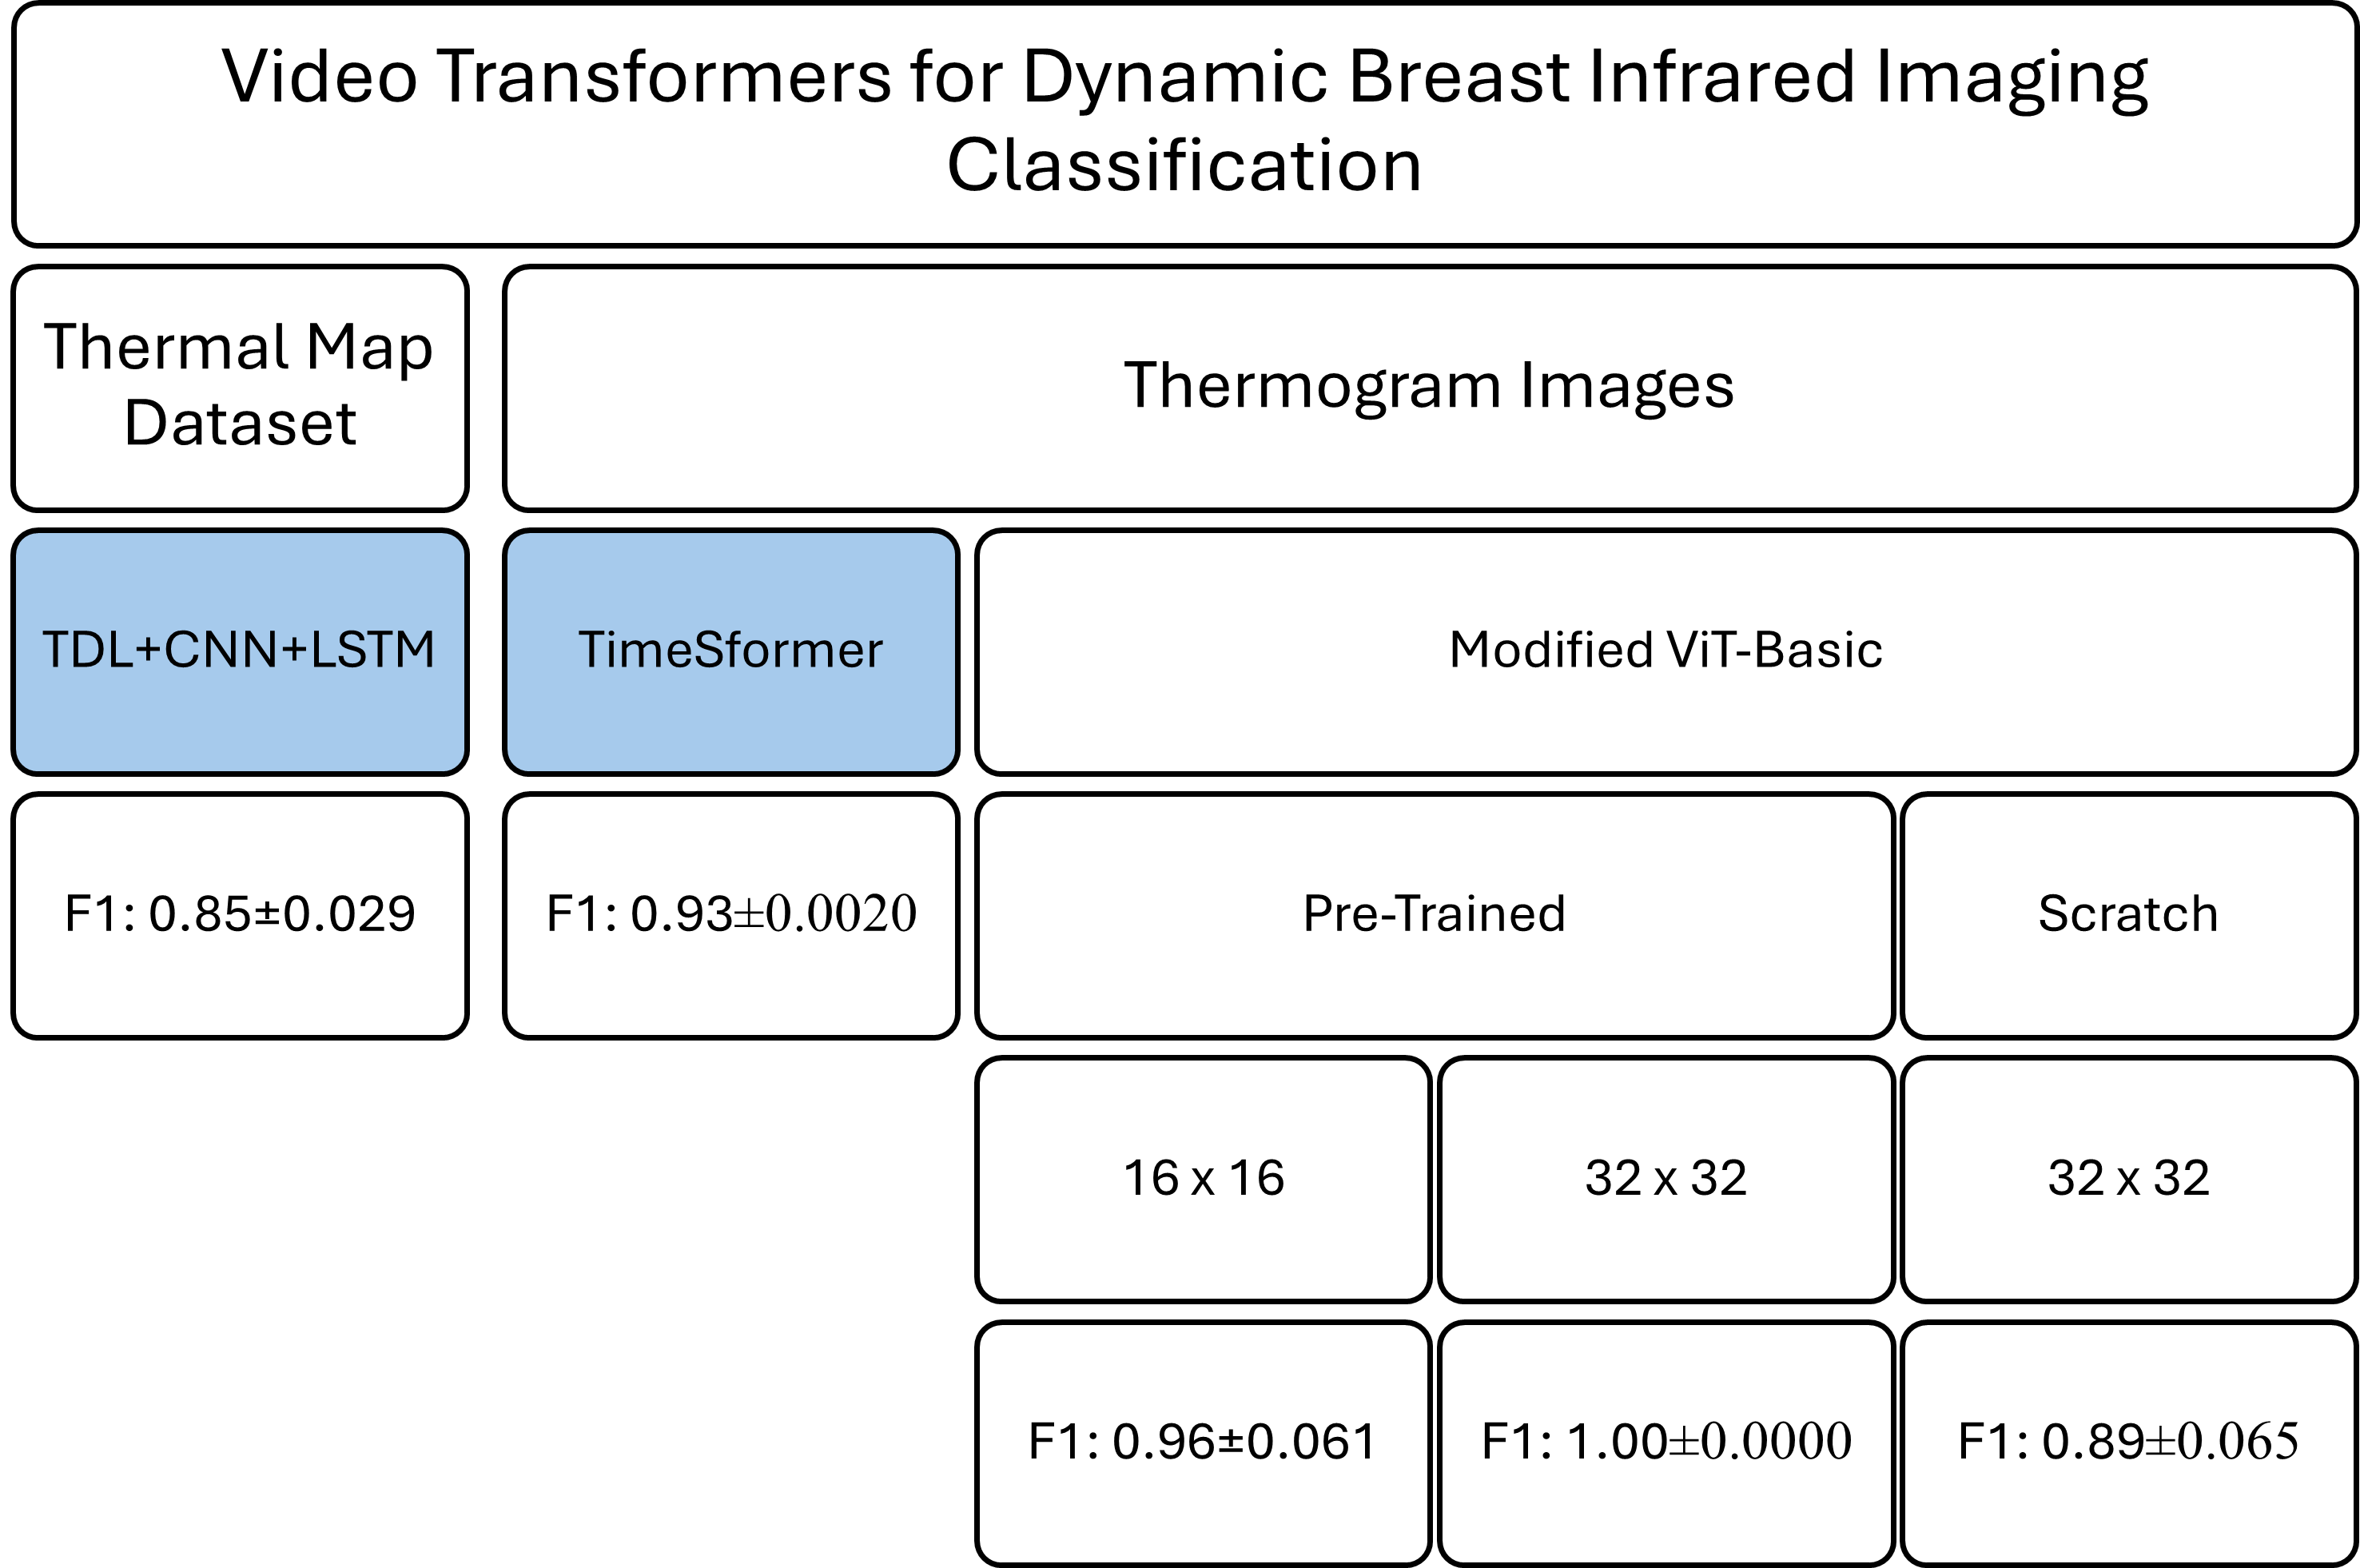
\includegraphics[scale=0.35]{figures/experimentalMethodologyGuide.png}
  \caption{A comparison of F1-score performance of all the Models for \ac{BC} in
    \ac{DIT} in this research. Highlighted are the sequential models
    like \ac{TDL} and \ac{ViViT} \label{fig:exp-guide} }
\end{figure}

\begin{table}[ht]
\centering
\caption{Training protocols for different modalities and architectures}
\label{tab:training_protocols}
\begin{tabular}{lllll}
\hline
\textbf{Modality} & \textbf{Model} & \textbf{Training Configuration} & \textbf{Validation} & \textbf{Epochs} \\
\hline
\ac{TM} & TDL+CNN+LSTM & AdamW, $k=3$ CV & Loss & 50 \\
\hline
\multirow{2}{*}{\ac{IR}} & \ac{ViT} (16$\times$16) pre-trained & AdamW, lr=3e-5, $k=10$ CV & F1-score & 20 \\
 & \ac{ViT} (32$\times$32) pre-trained & AdamW, lr=3e-5, $k=10$ CV & F1-score & 20 \\
\hline
\ac{IR} & \ac{ViT} (32$\times$32) scratch & \begin{tabular}[c]{@{}l@{}}AdamW, lr=1e-4, wd=0.05\\ LR warmup + cosine\\ (min lr=1e-6), $k=10$ CV\end{tabular} & Loss & 50 \\
\hline
\ac{IR} & \ac{ViViT} & AdamW, lr=3e-5, $k=10$ CV & F1-score & 20 \\
\hline
\end{tabular}
\end{table}

Our experimental protocol varied across modalities and
architectures. For \ac{TM} data, we employed 3-fold cross-validation
trained for 50 epochs using AdamW optimizer while monitoring
validation loss. For \ac{IR} images with pre-trained \ac{ViT} models
(both 16$\times$16 and 32$\times$32 patch sizes), we used 10-fold
cross-validation for 20 epochs with a \ac{lr} of 3e-5,
optimizing for validation F1-score. However, when training the
32$\times$32 patch \ac{ViT} from scratch, we extended training to 50
epochs with higher initial \ac{lr} (1e-4), weight decay (0.05),
and implemented \ac{lr} warmup with cosine annealing (minimum
lr=1e-6), while monitoring validation loss. The \ac{ViViT} model
followed similar configuration to pre-trained \ac{ViT}s (20 epochs,
lr=3e-5) monitored by F1-score. Table~\ref{tab:training_protocols}
presents the training protocols used for the different
modality-architecture combinations.

\section{Results}
\label{sec:results}
% **Results:** Present quantitative performance (tables and figures),
% comparative analysis, and discussion.
In this section, we discuss the quantitative performance of the
different models in our proposed experiments (Table \ref{tab:results})
and compare our work with the most relevant studies identified through
our literature review (Table \ref{tab:study_comparison}).

Our work is similar to that of Garia et al.~\cite{Garia2023} in the
use of Transformer-based models for breast cancer classification using
Thermography (\ac{TG}). However, we address dynamic infrared thermography
(\ac{DIT}), which requires a different methodological
focus. Specifically, we investigate: (1) a temporal deep learning
(\ac{TDL}) approach using Time Distributed Layer
(\ac{TDL})+\ac{CNNs}+\ac{LSTM}; (2) vision transformers (\ac{ViT}),
both with pre-trained weights and trained from scratch; and (3)
pre-trained video vision transformers (\ac{ViViT}).

Consequently, our problem is most similar to the work of Baffa et
al.~\cite{DeMatheus2023}. Unlike their approach, we propose the use of
pre-trained \ac{ViViT} TimeSformer to address the sequential nature of
\ac{DIT}. Our results indicate that \ac{ViViTs} exhibit performance
comparable to 3D-\ac{CNNs} for UFF's dynamic acquisition protocol in the
DMR-IR dataset. However, there are important differences with respect to
their work: (a) we work with a larger input tensor, providing higher
resolution (their work resizes inputs to $(B, 20, 32, 32, 3)$, while
we use $(B, 8, 224, 224, 3)$); (b) although the TimeSformer
architecture reduces the number of frames processed, the model
achieves similar performance.

Similar to Baffa et al., our unit of analysis is the patient, whereas
Garia et al. focus on individual images since they focus on \ac{SIT}
protocol. Experiments using the basic \ac{ViT} architecture show
performance comparable to \ac{ViViT}, specially when using
$32\times 32$ patches. But it is important to notice that \ac{ViT}
cannot process infrared (\ac{IR}) images sequentially because they are
inherently spatial and do not operate across the time dimension. As a
result, frames are effectively averaged during processing.

Finally, our results suggest that further investigation is required
when working directly with temperature matrices (\ac{TM}). We also
recommend that future research clearly indicate whether they are using
\ac{IR} images or raw temperature values.

\begin{table}[h]
  \centering
  \scriptsize
\caption{Performance comparison of different models on \ac{DIT} data}
\label{tab:results}
\begin{tabular}{lllll}
\hline
\textbf{Dataset} & \textbf{Model} & \textbf{Metric} & \textbf{Cross-Val (Mean $\pm$ Std)} & \textbf{Test Set} \\
\hline
\multirow{2}{*}{$\mathbb{D}_{\mathrm{TM}}$} & \multirow{2}{*}{TDL+CNN+LSTM} & F1-score & $0.8585 \pm 0.0296$ ($k=3$) & - \\
 & & AUC & - & - \\
\hline
\multirow{12}{*}{$\mathbb{D}_{\mathrm{IR}}$} & \multirow{3}{*}{ViT (16$\times$16) pre-trained} & F1-score & $0.9644 \pm 0.0458$ & - \\
 & & Accuracy & $0.9538 \pm 0.0615$ & 0.87 \\
 & & AUC & - & - \\
\cline{2-5}
 & \multirow{3}{*}{ViT (32$\times$32) pre-trained} & F1-score & $1.0000 \pm 0.0000$ & 0.9412 \\
 & & Accuracy & $1.0000 \pm 0.0000$ & 0.9333 \\
 & & AUC & $1.0000 \pm 0.0000$ & 0.9444 \\
\cline{2-5}
 & \multirow{3}{*}{ViT (32$\times$32) scratch} & F1-score & $0.9101 \pm 0.0665$ & 0.8889 \\
 & & Accuracy & $0.8939 \pm 0.0652$ & 0.8667 \\
 & & AUC & $0.8866 \pm 0.0595$ & 0.8611 \\
\cline{2-5}
 & \multirow{3}{*}{ViViT} & F1-score & $0.9339 \pm 0.0020$ & 0.9412 \\
 & & Accuracy & $0.9231 \pm 0.0000$ & 0.9333 \\
 & & AUC & $0.9350 \pm 0.0094$ & 0.9444 \\
% \cline{2-5}
%  & \multirow{1}{*}{3D-CNN} & AUC & $0.9351 \pm 0.0403$ & - \\
\hline
\end{tabular}
\end{table}

\begin{table}[htbp]
  \centering
  \scriptsize
\caption{Comparison of studies on breast thermography classification}
\label{tab:study_comparison}
\begin{tabularx}{\textwidth}{l *{9}{>{\centering\arraybackslash}X}}
\toprule
\textbf{Study} & \textbf{Model} & \textbf{Protocol} & \textbf{Pre-trained} & \textbf{Dataset} & \textbf{Analysis Unit} & \textbf{Total Subjects} & \textbf{Cross Validation} & \textbf{Test Set} & \textbf{AUC} \\
\midrule
Garia et al~\cite{Garia2023} & ViT & SIT & No & DMR-IR & Images & 950 & - & 10\% & 0.9570 \\
Baffa et al~\cite{DeMatheus2023} & 3D-CNN & DIT & No & DMR-IR & Patient & 149 & K=10 & - & 0.9351 \\
Our work & ViViT & DIT & Yes & DMR-IR & Patient & 149 & K=10 & 10\% & \textbf{0.9444} \\
\bottomrule
\end{tabularx}
\end{table}
\newpage
\section{Discussion}
\label{sec:discussion}
To the best of our knowledge, this work presents the first application
of a \ac{ViViT} to the \ac{DIT} protocol. Our approach achieves
superior performance on a test set of 15 patients (93\% accuracy, 93\%
precision, 94\% recall) compared to the results reported in
\cite{DeMatheus2023}. Furthermore, in a $K=10$ cross-validation
setting, our method achieves a similar mean accuracy of 93.50\% but
demonstrates superior stability, as indicated by a significantly
smaller standard deviation of $\pm$ 0.94\%. This higher precision and
lower variance suggest a more robust model. It is noteworthy that our
experiments utilize \ac{IR} images with a spatial resolution of
$224 \times 224$ pixels, a significantly larger input size compared to
the $32 \times 32$ images used by the baseline method in
\cite{DeMatheus2023}. We employ a shorter temporal sequence ($F=8$
frames) to accommodate the use of a pre-trained model. To address
this, future ablations studies should quantify the incremental value of
temporal modeling by varying (a) the number of frames (e.g., 3, 4, 6,
8, and the full 20-frame sequence), (b) the sampling strategy
(contiguous vs.\ uniformly spaced frames), and (c) the timing (early
vs.\ late frames relative to cooling).

Another important difference is that our current results do
not use a prior segmentation stage. Moreover, this arises the question
if segmentation would increase performance in our results. However, as
indicated in~\cite{Ryan2025}, there are no ablation studies that could
confirm this in infrared \ac{TG}.

Our experiments corroborate that \ac{ViTs} with $32 \times 32$ patches
yield better performance. However, it should be noted that a different
acquisition protocol for the same dataset was employed compared to
\cite{Garia2023}. In contrast to their findings, pre-training clearly
benefited performance in our experiments, despite the domain gap between
natural images/videos and medical thermal data.

\ac{DIT} aims to capture physiological responses under thermal stress
that may not be visible in single static frames. Our results show that
a pre-trained spatial \ac{ViT} with temporal averaging can reach
performance comparable to a pre-trained video transformer, suggesting
that a substantial portion of the discriminative signal may be
spatial. This raises two complementary questions: (i) whether the
current \ac{DIT} protocol sufficiently captures the
temporal dynamics it is designed to measure, and (ii) whether simpler
static protocols (\ac{SIT}) augmented with robust spatial modeling could be
adequate for certain clinical scenarios.

The results also suggest that future works should emphasize the type
of thermal data used, as outcomes obtained directly from the point
temperatures in CSV files differ from those using \ac{IR} images. The
challenges associated with temperature maps may stem from the fact
that pre-trained networks are typically trained on natural images,
which constitute a domain distinct from both \ac{IR} imagery and
temperature maps. We observed that infrared RGB images delivered
stronger performance than raw temperature matrices.
\newpage
\subsection{Threats to Validity}
\label{sec:threats-validity}

Our study is primarily limited by: (i) the relatively small size of
the dataset, and (ii) the absence of clinical validation. Although
this research prevented patient information leakage in the hold-out
test set, the limited sample size, combined with the use of large
architectures such as transformers, increases the risk of
overfitting. This risk, in turn, limits the potential for the clinical
translation of these results. To mitigate overfitting, \ac{FT} and
data augmentation were employed; however, future work should include
statistical tests and ablation studies to further validate and improve
the model's performance. The sample size of available public datasets,
however, is a factor over which we have limited control, besides some
of the suggestions indicated in~\cite{Ryan2025}. Clinical validation,
while challenging to achieve, is necessary. It would not only validate
the current model but also enhance it by incorporating other
physiological factors (e.g., menstrual cycle, hormone therapy) that
may influence thermographic patterns and, consequently, the model's
performance.


\section{Conclusions}
\label{sec:conclusions}

This research paper shows that \ac{ViViTs} can be effectively applied
to \ac{BC} classification using dynamically acquired \ac{TG}
images. Our current results show that the basic TimeSformer with 8
frames has achieved a similar performance to 3D-CNN in a prior
work. Also, this work extends that of~\cite{Garia2023} by extending to
the dynamic protocol.

With respect to the research questions, we conclude that
transformer-based models exhibit a performance comparable to that of
\ac{CNNs} for this research problem. In our experiments, fine-tuning a
pre-trained model yielded superior performance. Finally, the
integration of \ac{DIT} with \ac{ViViTs} achieves results similar to
those reported in~\cite{Garia2023}. Moreover, our results indicate
that \ac{ViTs} with temporal averaging perform similarly to fine-tuned
\ac{ViViTs}. This suggests that further research is necessary to fully
account for the effect of temporal dynamics in \ac{BC} prediction
using infrared images and transformer-based architectures.


% ==================== original conclusion section ====================
% To the best of our knowledge, this work presents the first application
% of a \ac{ViViT} to the \ac{DIT} protocol. Our approach achieves
% superior performance compared to the results reported in
%~\cite{DeMatheus2023} on a test set of 15 patients, while yielding
% comparable outcomes in a $K=10$ cross-validation setting. It is
% noteworthy that our experiments utilize \ac{IR} images with a spatial
% resolution of $224 \times 224$ pixels, a significantly larger input
% size compared to the $32 \times 32$ images used by the baseline method
% in~\cite{DeMatheus2023}, although we employ a shorter temporal
% sequence ($F=8$ frames).

% Our experiments corroborate that \ac{ViTs} with $32 \times 32$ patches
% yield better performance. However, it should be noted that we have
% used a different acquisition protocol of the same dataset wrt. to
%~\cite{Garia2023}. In contrast to their results, training from scratch
% underperformed in our setup.

% Consequently, we infer that \ac{ViViTs} can be applied with a good
% performance in \ac{BC} classification with \ac{TG} images acquired
% dynamically. Our experiments also suggest that future works should
% emphasize on what type of thermal data was used in the experiments
% since results using directly the point temperatures of the CSV files
% are different from those when using \ac{IR} images.

% With respect to the research questions, we conclude that
% transformer-based models exhibit a performance comparable to that of
% \ac{CNNs} for this research problem. In our experiments, fine-tuning a
% pre-trained model yielded superior performance. Finally, the
% integration of \ac{DIT} with \ac{ViViTs} achieves results similar to
% those reported in~\cite{Garia2023}.
% ==================== ==================== ====================


% % ==================== credits ====================
\begin{credits}
  \subsubsection{\ackname} Maria Pérez, Marco E. Benalcázar and Lenin
  G. Falconi would like to thank the support of Escuela Politécnica
  Nacional for the funding of this research. Aura Conci thanks the
  Brazilian agencies (FAPERJ and CNPq) for funding this research at
  UFF (307638/2022-7 and E26/200.924/2022).

% bold run-in heading in small font size at the end of the paper is
% used for general acknowledgments, for example: This study was funded
% by X (grant number Y).

  \subsubsection{\discintname}
  The authors have no competing interests to declare that are relevant
  to the content of this article
% It is now necessary to declare any competing interests or to specifically
% state that the authors have no competing interests. Please place the
% statement with a bold run-in heading in small font size beneath the
% (optional) acknowledgments\footnote{If EquinOCS, our proceedings submission
% system, is used, then the disclaimer can be provided directly in the system.},
% for example: The authors have no competing interests to declare that are
% relevant to the content of this article. Or: Author A has received research
% grants from Company W. Author B has received a speaker honorarium from
% Company X and owns stock in Company Y. Author C is a member of committee Z.
\end{credits}
% ==================== credits ====================
% 
% ---- Bibliography ----
%
% BibTeX users should specify bibliography style 'splncs04'.
% References will then be sorted and formatted in the correct style.
%
\newpage
\bibliographystyle{splncs04}
\bibliography{bibliography}

\end{document}

%%% Local Variables:
%%% mode: LaTeX
%%% TeX-master: t
%%% End:
